\section{Implement Gradient Descent}
\subsection{Implementation the gradient Descent}
We implemented a function {\tt gradientDescent}  that takes the parameters:
\begin{enumerate}[-]
\item A scalar function $f: \mathbb{R}^n \mapsto \mathbb{R}$.
\item The gradient of $f$ $\nabla f: \mathbb{R}^n \mapsto \mathbb{R}^n$.
\item An initial guess $x \in \mathbb{R}^n$.
\item A step size $s > 0$.
\item A convergence threshold $\epsilon > 0$.
\end{enumerate}
 {\tt gradientDescent} returns an array of $n+1$ numbers, corresponding to the $n$ coordinates of the current $x_t$, and the value of $f(x_t)$, for each of the steps $t$ before convergence of the algorithm.
 
 This choice of output lets us monitor the rate of convergence of the algorithm (which zones lead to slower or faster convergence), which will be useful when we compare different methods (see section \ref{comparison}). It also allows us to plot the path followed by the algorithm (see figures \ref{} to \ref{}).

\subsection{Benchmark and Choice of the parameters}

We chose to benchmark our gradient descent on a variety of functions, designed to test all the potential cases that we might encounter. Because of plotting constraints, we focus the figures to function of two parameters:  $f: \mathbb{R}^2 \mapsto \mathbb{R}$.

\begin{figure}[h!]
  \centering
 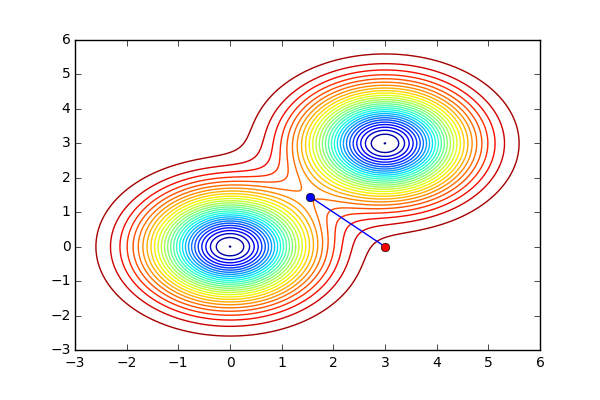
\includegraphics[width=8cm]{../Figures/Q1/normals.png}
\caption{$f : (x,y) \to e^{-\frac{x^2 + y^2}{2}} + e^{-\frac{(x-3)^2 + (y-3)^2}{2}}$}
\label{wtime}
\end{figure}
\begin{figure}[h!]
  \centering
 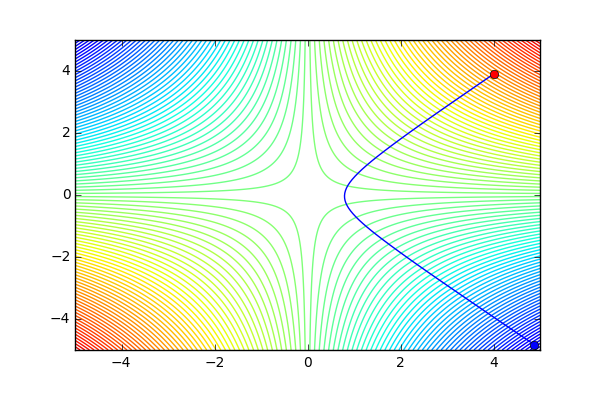
\includegraphics[width=8cm]{../Figures/Q1/nonconv.png}
\caption{$f : (x,y) \to xy$}
\label{wtime}
\end{figure}
\begin{figure}[h!]
  \centering
 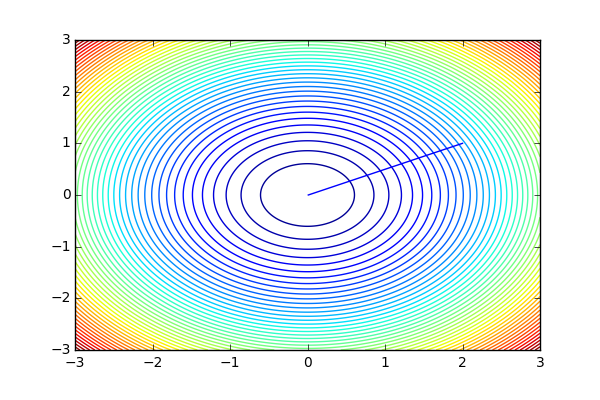
\includegraphics[width=8cm]{../Figures/Q1/bowl.png}
\caption{$f : (x,y) \to x^2 + y^2$}
\label{wtime}
\end{figure}


\subsection{Numerical Gradient}
\subsection{Comparison with existing optimization methods}
\label{comparison}